\documentclass{article}
\usepackage[T1]{fontenc}
\usepackage[utf8]{inputenc}
\newcommand{\myname}{Amit Rajaraman}
\newcommand{\topicname}{The sum-of-squares method}
\usepackage{../generic}

\newcommand{\pge}{\succeq} % poset le
\newcommand{\pg}{\succ} % poset le
\newcommand{\ple}{\preceq} % poset le
\newcommand{\size}{\operatorname{size}}
\newcommand{\vol}{\operatorname{vol}}
\newcommand{\pE}{\widetilde{\E}}
\newcommand{\opt}{\mathsf{opt}}
\newcommand{\aGW}{\alpha_{\text{GW}}}
\newcommand{\SOS}{\text{SOS}}
\newcommand{\supp}{\operatorname{supp}}

\begin{document}

\thispagestyle{empty}

\titleBC
\tableofcontents
\clearpage

\setcounter{section}{-1}
\section{Notation and Prerequisites}
	
	Given $n \in \N$, $[n]$ denotes the set $\{1,\ldots,n\}$ and $[n]_0$ denotes the set $[n] \cup \{0\}$.\\
	$S(n,k)$, a Stirling number of the second kind, is the number of partitions of $[n]$ into exactly $k$ parts. $s(n,k)$, a Stirling number of the first kind, is the number of permutations of $[n]$ with exactly $k$ cycles.\\
	
\clearpage
%!TEX root = ./main.tex

\section{Fundamentals}

\subsection{Introduction}

	Consider the problem of, for a given multivariate polynomial $p$, determining whether $p(x) \ge 0$ for $x$ in some (subset of) $\R^n$. It is not difficult to see that this can capture a huge spectrum of problems, specifically NP-hard ones such as max-cut -- given a graph $G$ on $n$ vertices, consider the polynomial $f : \{-1,1\}^n \to \R$ defined by
	\[ f(x) = \sum_{ij \in E} (x_i - x_j)^2. \]
	Then, there exists $x$ such that $f(x) \le k$ -- or equivalently, the polynomial $k - f(x)$ is non-negative on $\{-1,1\}^n$ -- iff every cut is of size at most $k$.\\
	So, this problem of determining non-negativity of a polynomial is NP-hard. What next?\\

	The sum-of-squares technique, at its most basic form, is a a restriction to a certain type of non-negativity. For now, suppose that our ``base set'' is $\{0,1\}^n$. \\
	More concretely, we shall show non-negativity by expressing $p$ as a \emph{sum of squares} of \emph{low degree} polynomials (while low degree is not technically required, the resulting algorithm need not be efficient otherwise).
	\begin{fdef}[Sum-of-squares proof]
		\label{def:sos}
		Given a polynomial $f \in \R[x_1,\ldots,x_n]$, a \emph{degree $d$ sum-of-squares proof} or \emph{degree $d$ sum-of-squares certificate} (abbreviated SoS proof or SoS certificate) of $f \ge 0$ is a set $\{g_1,\ldots,g_m\}$ of polynomials of degree at most $d/2$ such that
		\begin{equation}
			\label{eqn: base-sos}
			f(x) = \sum_{i=1}^m g_i^2(x)
		\end{equation}
		as polynomials.
		If $f$ has a degree $d$ sum-of-squares certificate, we write that
		\[ \sststile{x}{d} f(x) \ge 0. \]
		Let $\mathcal{A}$ be a set of constraints of the form $f_i(x) \ge 0$ for $i \in [m]$. Then, an \emph{degree $d$ SoS proof given $\mathcal{A}$} of $f \ge 0$ is a set $\{p_S\}_{S \subseteq [m]}$ of degree $d$ sum-of-squares polynomial (in the sense that it satisfies \Cref{eqn: base-sos} for some $(g_i)$), where $S$ ranges over \emph{multi}sets of elements in $[m]$ such that
		\[ f(x) = \sum_{S \subseteq [m]} p_S(x) \prod_{i \in S} f_i(x) \]
		as polynomials. If this is the case, we write
		\[ \mathcal{A} \sststile{x}{d} f \ge 0. \]
	\end{fdef}
	We always assume that $d$ in this context is even. We often suppress the variable $x$, and rarely even the degree $d$, in the above notation if they are clear from context. \\
	Although $\mathcal{A}$ contains only inequalities of polynomials, we can easily also make it contain equalities of polynomials by adding two corresponding constraints -- for $p(x) = k$, add $p(x)-k \ge 0$ and $k-p(x) \ge 0$. \\

	Note that simple set restrictions can be captured by the set of constraints. In particular, we can check restrict ourselves to the boolean hypercube $\{-1,1\}^n$ by having $\mathcal{A}$ contain $x_i^2 = 1$ for all $i$. Other than this, the reader can more or less ignore the second part of the above definition until \Cref{sec:constrained}, where we shall use its power in more depth.
	Also observe that the set of functions with degree $d$ SoS proofs of non-negativity forms a closed convex cone.

	\begin{fprop}
		\label{prop: deg-2n-sos}
		Any non-negative $f : \{-1,1\}^n \to \R$ has a degree $2n$ sum-of-squares proof.
	\end{fprop}
	\begin{proof}
		Recall that any function $h : \{-1,1\}^n \to \R$ can be expressed as a polynomial of degree at most $n$ as
		\[ h(x) = \sum_{S \subseteq [n]} \hat{f}(S) x_S, \]
		where $x_S = \prod_{i \in S} x_i$ with the convention $x_\emptyset = 1$. Knowledgeable readers may recognize this as the \emph{Fourier expansion} of $h$ -- we omit the details of why such an expansion exists, but refer the reader to the excellent text by O'Donnell \cite{bfa_od} for more details. In particular, $\sqrt{f}$ is a polynomial of degree at most $n$, so squaring both sides we get that $f$ has a degree $2n$ SoS proof.
	\end{proof}

	The above is \emph{not} true in general; not every non-negative polynomial $f : \R^n \to \R$ can be written as a sum of squares.

	\begin{definition}
		Given a vector $y \in \R^n$, the vector $y^{\otimes k} \in \R^{n^d}$ has entries indexed by elements of $[n]^d$, with the $\alpha$th entry being $\prod_{j \in d} y_{\alpha_j}$. Also denote $v_k(x)$ to be the size $\binom{n+k}{k}$ vector with entries equal to all the monomials of $x$ of degree at most $k$.
	\end{definition}
	Note that for $x \defeq (x_1,\ldots,x_n) \in \R^n$, any monomial of degree at most $d/2$ appears in the vector $(1,x)^{\otimes d/2}$, where $(1,x) = (1,x_2,\ldots,x_n) \in \R^{n+1}$. Also recall that a matrix $A$ is said to be positive semidefinite, denoted $A \pge 0$, if $x^\top A x \ge 0$ for all vectors $x$, which is equivalent to asserting that all eigenvalues of the matrix are non-negative.

	\begin{fprop}
		\label{prop: sos-sdp-equiv}
		Let $f$ be a polynomial. $f$ has a degree $d$ sum-of-squares proof iff there exists $A \pge 0$ such that
		\begin{equation}
			\label{eqn: sos-sdp-equiv}
			f(x) = \langle  v_{d/2}(x) , A v_{d/2}(x) \rangle.
		\end{equation}
	\end{fprop}
	\begin{proof}
		For the forward direction, suppose that $f = \sum_{i=1}^m g_i^2$, with $g_i(x) = v_i^\top v_{d/2}(x)$ by writing it out in the monomial basis. Then,
		\begin{align*}
			f(x) &= \sum_{i=1}^{m} v_{d/2}(x)^\top v_i v_i^\top v_{d/2}(x) \\
				&= \left\langle v_{d/2}(x) , \underbrace{\sum_{i=1}^m v_iv_i^\top}_{A} v_{d/2}(x) \right\rangle.
		\end{align*}
		The backward direction is straightforward by decomposing $A$ as $\sum \lambda_i v_i v_i^\top$, where each $\lambda_i \ge 0$, and observing that each $v_i^\top v_{d/2}(x)$ is a polynomial of degree at most $d/2$.
	\end{proof}
	As a corollary, this implies that if an $f$ has a degree $d$ SoS proof, it has one with at most $\binom{n+d}{d}$ squares.
	Also note that \cref{eqn: sos-sdp-equiv} is \emph{linear} in the elements of $A$.

	If we bump up a function by enough, we can ensure non-negativity. It turns out that we can do the same to ensure SoS-ness.
	\begin{flem}
		\label{lem:large-enough-sos}
		Let $f:\{-1,1\}^n \to \R$ be any function of degree at most $d$. For sufficiently large $L$, $L+f$ has a degree $d$ SoS certificate.
	\end{flem}
	\begin{proof}
		Note that for any $S$, $1+x_S \ge 0$ has a degree $\left\lceil|S|/2\right\rceil$ SoS proof. Indeed, setting $S = T_1 \sqcup T_2$ for $T_1,T_2$ of (almost) equal size, $1+x_S = \frac{1}{2}(x_{T_1} + x_{T_2})^2$. Similarly, $1-x_S$ has a degree $|S|$ SoS proof as well. Therefore,
		\[ \sum_{|S| \le d} |\hat{f}(S)| + \sum_{|S| \le d} \hat{f}(S) x_S = \sum_{|S| \le d} |\hat{f}(S)|(1 + \sign(\hat{f}(S))x_S) \]
		has a degree $d$ SoS certificate, so the statement is true with $L = \sum_{|S| \le d} \hat{f}(S)$.
	\end{proof}

\subsection{Semidefinite Programming}

	The reader is likely familiar with \emph{linear programming}, where we are interested in
	\[ \min_{x \in \mathcal{P}} c^\top x, \text{ where } \mathcal{P} = \{ x \ge 0 : Ax = b \}. \]
	Although a linear program may in general have inequalities in the constraints, we may merge these into the $x \ge 0$ condition by introducing slack variables (if we have $\sum_i a_i x_i \ge 0$, we may add a non-negative variable $y$ and make it $\sum_i a_i x_i - y = 0$). In \emph{semidefinite programming}, the setting is mostly the same, albeit with the minor change that we represent the variables by a matrix instead of a vector, and we additionally have that this matrix is positive semidefinite. More concretely, denoting
	\[ \langle C,X\rangle = \sum_{i,j} C_{ij} X_{ij}, \]
	we are interested in
	\[ \min_{X \in \mathcal{S}} \langle C,X\rangle, \text{ where } \mathcal{S} = \{ X \pge 0 : \langle A_i,X\rangle = b_i \text{ for $i \in [m]$} \}. \]
	We interchangeably use $\mathcal{S}$ to denote the set of constraints and the corresponding body.
	\Cref{prop: sos-sdp-equiv} suggests a link between SoS proofs and SDPs. A natural question is: can we solve SDPs efficiently?\\
	Note that the set of all PSD matrices $X$ forms a convex cone. In combination with the linear constraints, the intersection of this cone and the affine subspace form a so-called ``spectrahedron'', which we would like to minimize our quantity over. Note that any linear program is a semidefinite program, by enforcing that all off-diagonal elements of the matrix are zero. To answer our earlier question, it turns out that we cannot solve SDPs exactly.\footnote{It is not even known if this is in \textsf{NP}! It is known that it is in \textsf{PSPACE} however.} However, if we enforce certain structural restrictions, we can solve them approximately (up to a small additive error).

	\begin{fdef}[Separation Oracle]
		For a convex body $K \subseteq \R^n$, a \emph{(strong) separation oracle} for $K$ does the following given as input any $x \in K$.
		\begin{enumerate}
			\item if $x \in K$, it returns \textsf{yes}.
			\item if $x \not\in K$, it returns \textsf{no}, and in addition a vector $a$ and real $b$ such that $\langle a,y\rangle \ge b$ for all $y \in K$ and $\langle a,x\rangle < b$  -- this is a so-called ``separating hyperplane'' that separates $x$ and $K$.
		\end{enumerate}
	\end{fdef}

	More generally, we can efficiently minimize an inner product over a convex (bounded) body up to an additive error of $\epsilon$, given an efficient weak separation oracle.

	\begin{ftheo}
		Let $f : \{-1,1\}^n \to \R$ have a degree $d$ sum-of-squares proof of non-negativity. Then, for $\epsilon > 0$, there exists an algorithm that finds a sum-of-squares proof of $f+\epsilon$ in $\poly(n^d,\log(1/\epsilon))$.
	\end{ftheo}

	The high-level idea of the algorithm is as follows.\\
	We first solve the ``feasibility problem'' of finding a point in a body $K$, given that $B(c,r) \subseteq K \subseteq B(0,R)$. We begin by setting $\mathcal{E}^{(0)} = B(0,R)$. Given the ellipsoid $\mathcal{E}^{(i)}$, if its center returns \textsf{yes}, we return the point itself. Otherwise, we use the separating hyperplane to get a halfspace $H$ in which $K$ is contained, and set $\mathcal{E}^{(i+1)}$ to be the smallest ellipsoid containing $\mathcal{E}^{(i)} \cap H$. This algorithm runs in $\poly(n,\size(K)) \log(R/r)$ -- the proof amounts to showing that the volume of the ellipsoid decreases by a factor of at least $\exp(1/2(n+1))$ at each stage, and we have a lower bound on the volume of $K$ by $\vol(B(0,r))$.\\
	We can slightly modify this algorithm to one that approximately solves the optimization version of maximizing $c^\top x$ as well. Once we get a point $\alpha$ in the body, we begin looking at $K \cap \{x : c^\top x > c^\top \alpha\}$ and repeat the feasibility algorithm. This is repeatedly done until we can guarantee that we are within $\epsilon$ of the optimum. The only non-trivial part of this algorithm is showing that we can use the oracle to construct an oracle for the new body $K \cap \{x : c^\top x > c^\top \alpha\}$.\\
	To complete the connection to SDPs, we require that the SDP constraints $\mathcal{S}$ admits an efficient weak separation oracle; we omit the details of this. Next, we require that the body $\mathcal{S}$ contains a ball and is contained in a ball. The former is not true in general because the constraints typically make our body lower-dimensional (a subspace). To get around this, we introduce an additive error in each the contraints, so the new constraints are $|\langle A,X\rangle - b_i| \le \epsilon$ for each $i$. In this case, there is a ball of radius $O( (\epsilon/\|A\|_F)^n )$ contained in the body, where $\|A\|_F^2 = \sum_{i,j,k} (A_i)_{jk}^2$.\\
	In our context of finding $X$ such that $f(x) = v_{d/2}(x)^\top X v_{d/2}(x)$, we know that $\|A\|_F^2 \le \Tr(A)^2 \le \hat{f}(\emptyset)^2$, so the body is bounded as well.\\

	Like how LPs have duals, so do SDPs. If we have the primal
	\[ \min_{X \in \mathcal{S}} \langle C,X\rangle , \text{ where } \mathcal{S} = \left\{ X \pge 0 : \langle A_i,X\rangle = b_i \text{ for $i \in [m]$} \right\}, \]
	its dual is
	\[ \max_{y \in \mathcal{S}^D} b^\top y, \text{ where } \mathcal{S}^D = \left\{ S \pge 0 : C - \sum_{i=1}^m y_i A_i = S \right\}. \]
	The PSDness condition in the dual just says that $C \pge \sum_{i=1}^m y_i A_i$.

	\begin{fprop}[Weak Duality]
		Let $X$ and $y$ be solutions to the primal and dual SDPs respectively. Then, $\langle C,X\rangle \ge b^\top y$.
	\end{fprop}
	\begin{proof}
		We have
		\begin{align*}
			\langle C,X\rangle &= \left\langle \sum_{i=1}^m y_i A_i + S , X \right\rangle \\
				&= \sum_{i=1}^m y_i \langle A_i,X\rangle + \langle S,X\rangle \\
				&= b^\top y + \langle S,X\rangle \ge b^\top y.
		\end{align*}
		The final inequality requires showing that if $S,X \pge 0$, then $\langle S,X\rangle \ge 0$ -- this is a simple corollary of the \nameref{schur-prod-thm} we shall see later, using $\mathbf{1}^\top (S \circ X) \mathbf{1} \ge 0$.
	\end{proof}

	In linear programming, we have strong duality which asserts that the two optima are in fact \emph{equal}. However, in SDPs, some mild conditions are required for this to be true. 

	\begin{ftheo}[Strong duality]
		Let $\mathcal{S}$ be the set of constraints of a primal SDP and $\mathcal{S}^D$ the set of constraints in its dual, such that the two have optima $\alpha^*,\beta^*$. Then, $\langle C,\alpha^*\rangle = \langle b,\beta^*\rangle$ if
		\begin{enumerate}
			\item the spectrahedron $\mathcal{S}$ is non-empty and there exists $\beta$ such that $\sum_{i \in [m]}\beta_i A_i - C \pg 0$, or
			\item the spectrahedron $\mathcal{S}^D$ is non-empty and there exists $\alpha \pg 0$ such that $ \langle A,\alpha\rangle = b_i$ for all $i \in [m]$.
		\end{enumerate}
		As a corollary, one may show that $\langle C,\alpha^*\rangle = \langle b,\beta^*\rangle$ if the set of optimal solutions of either of the two SDPs is non-empty and bounded.
	\end{ftheo}

	We omit the (rather involved) proof of the above.

\subsection{Pseudoexpectations}

	Let us again restrict ourselves to $\{-1,1\}^n$ for a while. We have established one link between SoS proofs and SDPs, and now we shall establish another link between them and the following.

	\begin{fdef}[Pseudodistribution]
		\label{def: pseudodistrib}
		A \emph{degree $d$ pseudodistribution} is a function $\mu : \{-1,1\}^n \to \R$ such that the expectation operator $\pE_{\mu}$ defined by $\pE_{\mu} f = \sum_{x \in \{-1,1\}^n} f(x) \mu(x)$ satisfies
		\begin{enumerate}[label=(\alph*)]
			\item $\pE_\mu 1 = 1$, and
			\item for all $f$ of degree at most $d/2$, $\pE_\mu f^2 \ge 0$.
		\end{enumerate}
		In this case, $\pE_\mu$ is called a \emph{pseudoexpectation}.
	\end{fdef}

	Analogous to \Cref{prop: deg-2n-sos}, we get that any degree $\ge 2n$ pseudodistribution is an actual distribution, in the sense that $\mu \ge 0$. Analogous to \Cref{prop: sos-sdp-equiv}, we get the following.

	\begin{fprop}
		\label{prop: pe-characterization}
		$\pE$ is a degree $d$ pseudoexpectation iff
		\begin{enumerate}[label=(\alph*)]
			\item $\pE 1 = 1$, and
			\item $\pE v_{d/2}(x) v_{d/2}(x)^\top \pge 0$. 
		\end{enumerate}
	\end{fprop}
	\begin{proof}
		Note that for any vector $(\hat{f})$ of Fourier coefficients of a degree $\le d/2$ function $f : \{-1,1\}^n \to \R$ (so $f(x) = \hat{f}^\top v_{d/2}(x)$),
		\begin{align*}
			\pE f^2 &= \pE \left(\sum_{|S| \le d} \hat{f}(S) x_S\right)^2 \\
				&= \pE \hat{f}^\top v_{d/2}(x) v_{d/2}(x)^\top \hat{f} \\
				&= \hat{f}^\top \left( \pE v_{d/2}(x) v_{d/2}(x)^\top \right) \hat{f}.
		\end{align*}
		To conclude, note that $\pE v_{d/2}(x) v_{d/2}(x) \pge 0$ iff $\hat{f}^\top \left( \pE v_{d/2}(x) v_{d/2}(x)^\top \right) \hat{f} \ge 0$ for all vectors $\hat{f}$.
	\end{proof}

	Given any function that is not non-negative everywhere, there exists some distribution $\mu$ such that $\E_\mu f < 0$. Ideally, we would like a similar result in order to distinguish between functions that have SoS certificates of degree $d$ and those that don't.

	\begin{ftheo}
		\label{theo: sos-pe-equiv}
		$f$ has a degree $d$ sum-of-squares proof iff for all degree $d$ pseudoexpectations $\pE$, $\pE f \ge 0$.
	\end{ftheo}
	Equivalently, $f$ does not have a degree $d$ sum-of-squares proof iff there exists a degree $d$ pseudoexpectation $\pE$ such that $\pE f < 0$.
	\begin{proof}
		The forward direction is straightforward by \Cref{def: pseudodistrib}(b). For the backward direction, suppose instead that $f$ does not have a degree $d$ SoS proof. Then, there exists a separating hyperplane between $f$ and this set, that is, some degree $d$ pseudoexpectation $\pE$ such that $\pE f < 0$. If we manage to show that $\pE 1 > 0$, we are done since we can then rescale $\mu$ to make it exactly equal to $1$. By \Cref{lem:large-enough-sos}, we have $L > 0$ such that $\pE (f+L) \ge 0$. Since $\pE f < 0$, this means that $\pE L = L \cdot \pE 1 > 0$, completing the proof.
	\end{proof}

	% Using our earlier discussion, given a function $f$,
	% \begin{enumerate}
	% 	\item if $f$ has a degree $d$ SoS certificate of positivity, we may establish so in $\poly(n^d,1/\epsilon,\size(f))$ time, and
	% 	\item if $f$ does not have a degree $d$ SoS certificate of positivity, we may find in $\poly(n^d,1/\epsilon,\size(f))$ time a pseudoexpectation $\pE$ such that $\pE f < \epsilon$.
	% \end{enumerate}
	Using our earlier discussion, given a function $f$ without a degree $d$ SoS certificate of positivity, we may find in $\poly(n^d,1/\epsilon,\size(f))$ time a pseudoexpectation $\pE$ such that $\pE f < \epsilon$.


%!TEX root = ./main.tex

\clearpage

\section{Degree $2$: Quadratic optimization on the hypercube}
\label{sec:quad-optim}

\subsection{Max-cut}
\label{subsec:max-cut}

	In this subsection, let us describe how the content of the previous three subsections interact through an example, and give an approximation algorithm for the max-cut problem.

	\begin{question*}
		Given a graph $G = (V,E)$, find $S \subseteq V$ such that the size of the cut $E(S,S^c) = \left\{ \{i,j\} \in E : i \in S, j \in S^c \right\}$ is maximized.
	\end{question*}

	Unlike min-cut, which may be solved in polynomial time using flow, the above is \textsf{NP}-complete.

	One basic approximation algorithm was proposed by Erd\H{o}s, which merely returns a random cut. With constant probability, the returned cut is a $1/2$-approximation of the max-cut. We shall in this algorithm study an algorithm due to Goemans and Williamson \cite{gw-maxcut}.\\
	Assume wlog that $V = [n]$, and identify any $S \subseteq V$ with the vector in $\{-1,1\}^n$ with a $1$ at precisely those vertices in $S$. Note that the function defined by
	\begin{equation}
		\label{eqn: fg-def}
		f_G(x) = \frac{1}{4} \sum_{ij \in E} (x_i - x_j)^2 = \frac{1}{2} \sum_{ij \in E} (1 - x_ix_j).
	\end{equation}
	on input $S$ returns precisely the size of the cut corresponding to $S$. Equivalently, considering the \emph{graph Laplacian} $L_G \defeq D_G - A_G$, where $D_G$ is the diagonal matrix of degrees and $A_G$ is the adjacency matrix, we have
	\begin{equation}
		\label{eqn: gw-lapl}
		f_G(x) = \frac{1}{4} x^\top L_G x.
	\end{equation}
	We are interested in $\max_{x \in \{-1,1\}^n} f_G(x) \eqdef \opt(G)$.
	%Now, inspired by SDPs, consider the relaxation where instead of looking at $\langle L,xx^\top\rangle$, we look at $\frac{1}{4}\langle L,X\rangle$ together with the constraint that $X \pge 0$. We also fix the diagonal entries of $X$ to be $1$.

	\begin{ftheo}
		\label{theo: gw-sos}
		Set $\aGW \defeq \min_{\rho \in [-1,1]} \frac{2\arccos(\rho)}{\pi(1-\rho)} \approx 0.8786$. Then,
		\[ \frac{\opt(G)}{\aGW} - f_G(x) \ge 0 \]
		has a degree $2$ sum-of-squares certificate.
	\end{ftheo}

	Let $\pE_\opt$ be a pseudoexpectation that maximizes $\pE_\opt f_G$ as $\opt_{\text{SOS}_2}(G)$. Clearly, $\opt_{\SOS_2}(G) \ge \opt(G)$. Furthermore, by the previous theorem,
	\[ \opt(G) \le \opt_{\text{SOS}_2}(G) \le \frac{1}{\aGW} \opt(G). \]
	By the discussion at the end of the previous subsection, we can find in $\poly(n,1/\epsilon)$ a degree $2$ pseudodistribution $\mu$ such that
	\[ \pE_\mu f_G \ge \opt_{\text{SOS}_2}(G) - \epsilon. \]
	So,
	\[ \frac{1}{\aGW} \opt(G) \ge \pE_\mu f_G \ge \opt(G) - \epsilon. \]

	\begin{flem}
		\label{lem: gw-pd-to-rd}
		Let $\mu$ be a degree $2$ pseudodistribution on $\{-1,1\}^n$. Then, there exists a (``real'') distribution $\mu'$ on $\{-1,1\}^n$ such that
		\[ \E_{\mu'} f_G \ge \aGW \cdot \pE_{\mu} f_G. \]
	\end{flem}
	Further, it is possible to efficiently sample from $\mu'$ given $\mu$. Plugging this back into our previous sequence of equations,
	\[ \E_{\mu'} f_G \ge \aGW(\opt(G) - \epsilon) \ge (\aGW - \epsilon) \opt(G), \]
	and efficient sampling implies that we can in $\poly(n,1/\epsilon)$ time sample a random cut $S$ such that with good probability, the size of the cut of $S$ is a $(\aGW-\epsilon)$-approximation of the max-cut.\\
	Let us now get to the proofs of the above results.

	\begin{proof}[Proof that \Cref{lem: gw-pd-to-rd} implies \Cref{theo: gw-sos}]
		It suffices to show that for all pseudodistributions $\pE_\mu$,
		\[ \pE_\mu \left[ \frac{\opt(G)}{\aGW} - f_G \right] \ge 0. \]
		Equivalently, we would like to show that
		\[ \pE_\mu f_G \le \frac{\opt(G)}{\aGW}. \]
		Letting $\mu'$ be a distribution as in \Cref{lem: gw-pd-to-rd},
		\[ \pE_\mu f_G \le \frac{1}{\aGW} \E_{\mu'} f_G \le \frac{1}{\aGW} \opt(G). \qedhere \]
	\end{proof}

	\begin{proof}[Proof of \Cref{lem: gw-pd-to-rd}]
		We may assume wlog that $\pE_\mu x = 0$, by changing $\mu(x)$ to $\frac{\mu(x) + \mu(-x)}{2}$ -- note that this procedure does not change $\pE_\mu f_G$ because $f_G(x) = f_G(-x)$. Using \Cref{prop: pe-characterization}(b) and recalling that any principal submatrix of a PSD matrix is PSD, $\pE_\mu xx^\top \pge 0$. So, let $\nu$ be a normal distribution on $\R^n$ with mean $0$ and covariance matrix $\pE_\mu xx^\top$. Finally, define $\mu'$ by the process that samples a vector $g$ according to $\nu$ and returns $\hat{x} = \sign(g)$, the vector in $\{-1,1\}^n$ whose $i$th coordinate is just the sign $\pm 1$ of $g_i$ -- this is well-defined with probability $1$. Note that an $(x_i - x_j)^2$ term in $f_G$ contributes to the cut iff $\sign(g_i) \ne \sign(g_j)$. That is,
		% box-muller transform can be used to get the gaussian
		\[ \E_{\mu'} f_G = \sum_{ij \in E} \Pr[\sign(g_i) \ne \sign(g_j)]. \]
		For distinct $i,j$, set $\rho_{ij} = \E_{\mu}[x_i x_j] = \E [g_i g_j]$. Let $h \sim \mathcal{N}(0,\Id_2)$. Then, to analyze the above probability (for a fixed $i,j$), we can assume that $g_i = \langle h,v\rangle$ and $g_j = \langle h,w\rangle$ for some $v,w$ such that $\langle v,w\rangle = \rho_{ij}$. So, $\sign(g_i) \ne \sign(g_j)$ iff $\langle h,v\rangle$ and $\langle h,w\rangle$ have opposite signs. Because the ``direction'' $h/\|h\|$ of $h$ is uniformly distributed on $\mathbb{S}^1$, we get that
		\[ \Pr[\sign(g_i) \ne \sign(g_j)] = \frac{\arccos(\rho_{ij})}{\pi}, \]
		as seen in the following diagram, where $h$ must lie in the green region for the signs to be different.

		\begin{center}
		% \centering
		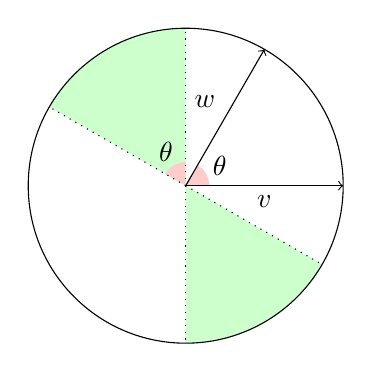
\begin{tikzpicture}
			\path[fill=green!20] (0,0) -- +(90:2) arc (90:150:2) -- (0,0);
			\path[fill=green!20] (0,0) -- +(-90:2) arc (-90:-30:2) -- (0,0);
			\coordinate (o) at (0,0);
			\coordinate (v) at (0:2);
			\coordinate (w) at (60:2);
	        \path[fill=red!20] (o) -- ++(60:.3) arc (60:0:.3) -- (o);
	        \path[draw] ++(30:.5) node {$\theta$};
	        \path[fill=red!20] (o) -- ++(90:.3) arc (90:150:.3) -- (o);
	        \path[draw] ++(120:.5) node {$\theta$};
	        \draw[dotted] (o) -- (90:2);
	        \draw[dotted] (o) -- (150:2);
	        \draw[dotted] (o) -- (-30:2);
	        \draw[dotted] (o) -- (-90:2);
			\draw[->] (0,0) coordinate (O) -- (0:2) coordinate (v) node[midway,below] {$v$};
			\draw[->] (0,0) coordinate (O) -- (60:2) coordinate (w) node[midway,above left] {$w$};
			\draw (0,0) circle (2 cm);
		\end{tikzpicture}

		The angle between $v,w$ is $\theta = \arccos(\rho_{ij})$.%\\So, $\Pr[\sign(\langle h,v\rangle) \ne \sign(\langle h,w\rangle)]$ is precisely $\theta/\pi$.
		\end{center}

		Using the facts that $\E[g_i^2] = 1$ and $\E[g_ig_j] = \rho_{ij}$, we have that $\E[(g_i - g_j)^2] = 2(1-\rho_{ij})$ and so
		\begin{align*}
			\E_{\mu'} f_G &= \sum_{ij \in E} \Pr[\sign(g_i) \ne \sign(g_j)] \\
				&= \sum_{ij \in E} \frac{\arccos(\rho_{ij})}{2\pi(1-\rho_{ij})} \E[(g_i - g_j)^2] \\
				&\ge \frac{\aGW}{4} \cdot \E\left[\sum_{ij \in E} (g_i - g_j)^2\right] = \aGW \pE_{\mu} f_G. \qedhere
		\end{align*}
	\end{proof}

	Now, we have managed to get roughly an $\aGW$-approximation using degree $2$ SoS. Is it possible to do any better using degree $2$ SoS? What about with a higher (but constant) degree? It might even be interesting to see if we can get a better approximation with non-constant degree, say $O(\log n)$.\\
	To answer the first question, it turns out that what we have done is indeed the best possible. There is also strong reason to believe that an $(\aGW+\epsilon)$-approximation is \textsf{NP}-hard, assuming the \emph{Unique Games Conjecture}, that we shall study in more detail in \Cref{subsec:ugc}.\\

	Let us get back to the Goemans-Williamson algorithm. Instead of looking at the best approximation ratio, can we parametrize the output result in terms of the optimal value?

	\begin{fprop}
		\label{prop: gw-reparametr}
		Let $G$ be a graph with $\opt(G) = (1-\delta)|E|$. For the output distribution $\mu'$ of the Goemans-Williamson algorithm, $\E_{\mu'} f_G \ge (1 - \sqrt{\delta}) |E|$.
	\end{fprop}
	\begin{proof}
		Let
		\[ h_G(x) = |E| - f_G(x) = \frac{1}{2} \sum_{ij \in E} 1+x_ix_j. \]
		It suffices to show that given a degree $2$ pseudodistribution $\mu$ such that $\pE_\mu h_G = \delta |E|$, there exists a distribution $\mu'$ such that $\E_{\mu'} h_G \le \sqrt{\delta} |E|$. This distribution $\mu'$ is defined exactly the same as in the Goemans-Williamson algorithm.  We denote $g$ and $\hat{x}$ as we do in the proof.
		Letting $\rho_{ij} = \E g_i g_j = \pE_\mu x_i x_j$, recall from the proof of \Cref{lem: gw-pd-to-rd} that $\E \hat{x}_i \hat{x}_j = \frac{2}{\pi} \arcsin \rho_{ij}$. This implies that
		\[ \E_{\mu'} h_G = \E_{\mu'} \sum_{ij \in E} \frac{1+\hat{x}_i \hat{x}_j}{2} = \frac{1}{2} \sum_{ij \in E} 1 + \frac{2}{\pi} \arcsin(\rho_{ij}). \]
		Also note that
		\begin{equation}
			\label{eqn: 2.2}
			\sup_{\rho \in [-1,1]} \frac{\left(1+(2/\pi)\arcsin(\rho)\right)^2}{1+\rho} = 2.
		\end{equation}
		Consequently,
		\begin{align*}
			\left(\E_{\mu'} h_G\right)^2 &= \frac{1}{4} \left(\sum_{ij \in E} 1+\frac{2}{\pi} \arcsin(\rho_{ij})\right)^2 \\
				&\le \frac{|E|}{4} \sum_{ij \in E} \left( 1 + \frac{2}{\pi} \arcsin(\rho_{ij}) \right)^2 \qquad\qquad \text{(Cauchy-Schwarz)} \\
				&\stackrel{\eqref{eqn: 2.2}}{\le} \frac{|E|}{2} \sum_{ij \in E} 1+\rho_{ij} \\
				&= |E| \cdot \E\left[\sum_{ij \in E} \frac{1+g_ig_j}{2}\right] \\
				&= |E| \cdot \pE_\mu h_G = \delta |E|^2,
		\end{align*}
		so $\E_{\mu'} h_G \le \sqrt{\delta} |E|$, completing the proof.
	\end{proof}

	Is this rounding we have done, called ``Gaussian rounding'', the best possible? It turns out that it is not, and we can in general do better using the ``RPR$^2$'' scheme of roundings. We shall soon study this in more detail.\\

	Let us now return to our earlier statement that it is impossible to do better using degree $2$ SoS. That is, for graphs in general, if we can get a degree $2$ SoS certificate of non-negativity for
	\[ \frac{\opt(G)}{c} - f_G(x), \]
	how large can $c$ be? We shall show that $c = \aGW$ is optimal, by looking at the cycle $C_n$ for odd $n$. This serves as a ``gap'' example. It is easily seen that the max-cut in this graph is $n-1 = \left( 1 - \frac{1}{n} \right) |E|$. We shall show that there exists a degree $2$ pseudodistribution $\mu$ such that
	\[ \pE_\mu f_{C_n} \ge \left( 1 - O\left(\frac{1}{n^2}\right) \right) |E|. \]
	Due to \Cref{prop: gw-reparametr}, this shows that the Goemans-Williamson algorithm is tight, at least up to constant factors. We can think of the cycle as something of a discretization of the $2$-dimensional sphere. If we instead look at the discretization of a high-dimensional sphere, it can be shown that this is tight even up to constant factors. We refer the reader to \cite{gw-tight-feige-schechtman} for details. The sketch of the proof for the cycle is as follows.\\
	Recall \cref{eqn: gw-lapl}, so we are interested in $\max_{x \in \{-1,1\}^n} x^\top L_G x$. This is at most $\max_{x : \|x\|_2 = \sqrt{n}} x^\top L_G x = n\|L_G\|_2$, which can be computed in polynomial time. Now, how do we construct a pseudodistribution $\pE$ for the cycle as mentioned earlier? Note that a given $\pE$ is a well-defined degree $2$ pseudodistribution iff $\pE (1,x) (1,x)^\top$ is a PSD matrix with $1$s on the diagonal. Now,
	\begin{align*}
		\pE f_G(x) &= \pE x^\top L_G x \\
			&= \pE \langle L_G , xx^\top \rangle \\
			&= \left\langle L_G , \pE xx^\top \right\rangle.
	\end{align*}
	Observe that the top eigenvalue of $L_G$ is indeed $1 - O(1/n^2)$, and this eigenspace is $2$-dimensional. It turns out that for an appropriate choice of $v_1,v_2$ in this eigenspace, we can ensure that $v_1v_1^\top + v_2v_2^\top$ does have only $1$s on the diagonal (this is essentially a consequence of the fact that $\sin^2\theta+\cos^2\theta = 1$).

\subsection{The positive semidefinite case}

	In the previous subsection, we looked at $\max_{x \in \{-1,1\}^n} x^\top L_G x$, where $L_G$ is the (positive semidefinite) Laplacian of a graph. This is an example of quadratic optimization, where we are more generally interested in
	\[ \opt(B) \defeq \max_{x \in \{-1,1\}^n} x^\top B x \]
	for some $n \times n$ matrix $B$.\\
	In the case where $B \pge 0$, it turns out that we can do something similar to what we had done in the max-cut algorithm.
	% -- it is possible to get a $\pi/2$-approximation, due to Nesterov \cite{quad-optim-psd}.

	\begin{ftheo}[Nesterov]
		\label{thm: nesterov}
		Let $B$ be a positive semidefinite $n\times n$ matrix. Then,
		\[ \frac{\opt(B)}{c} - x^\top B x \]
		has a degree $2$ sum-of-squares certificate for $c = 2/\pi \approx 0.63$.
	\end{ftheo}
	By the discussion in the previous section, this means as a corollary that we have a $\poly(n,1/\epsilon)$-time $(2/\pi-\epsilon)$-approximation algorithm for any $\epsilon > 0$.

	\begin{definition}
		Let $M \in \R^{n \times n}$. Given $f : \R \to \R$, define $f[M] \in \R^{n \times n}$ by $f[M]_{ij} = f(M_{ij})$ for all $i,j$.
	\end{definition}

	\begin{fprop}
		\label{prop: taylor-fM-psd}
		Suppose $M$ is a positive semidefinite matrix and $f$ a function whose Taylor series has all positive Taylor coefficients and is uniformly convergent on $[-1,1]$. Then, $f[M]$ is positive semidefinite.
	\end{fprop}

	The above is a corollary of the following simple observation.

	\begin{prop}[Schur Product Theorem]
		\label{schur-prod-thm}
		Let $M,M'$ be positive semidefinite matrices. Denote by $M \circ M'$ the \emph{Hadamard product} of $M,M'$ defined by $(M\circ M')_{ij} = M_{ij} M'_{ij}$. Then, $M \circ M'$ is positive semidefinite.
	\end{prop}
	\begin{proof}
		Let $M = \sum_i \lambda_i v_i v_i^\top$ and $M' = \sum_j \lambda_j' v_j'v_j'^\top$. Using linearity of the Hadamard product,
		\[ M \circ M' = \sum_{i,j} \lambda_i \lambda'_j (v_i v_i^\top) \circ (v_j v_j'^\top) = \sum_{i,j} \lambda_i \lambda'_j (v_i \circ v_j') (v_i \circ v_j')^\top \pge 0. \qedhere \]
	\end{proof}

	\begin{proof}[Proof of \Cref{prop: taylor-fM-psd}]
		Denote $[M]^2 = M \circ M$, and $[M]^i = [M]^{i-1} \circ M$ more generally. By the \nameref{schur-prod-thm}, $[M]^i \pge 0$ for all $i$. Therefore, $\sum c_i [M]^i \pge 0$, that is, $(\sum c_i x^i)[M] \pge 0$.
	\end{proof}

	% A straightforward corollary of \Cref{prop: taylor-fM-psd} is that $\arcsin[M] \pge M$.

	\begin{proof}[Proof of \nameref{thm: nesterov}]
		As in the previous subsection, let $\mu$ be a zero mean degree $2$ pseudodistribution on $\{-1,1\}^n$, $g$ a normal random variable with zero mean and covariance matrix $\pE_\mu xx^\top$, and $\hat{x} \defeq \sign(g)$ distributed as $\mu'$. A straightforward byproduct of the final part of the proof of \Cref{lem: gw-pd-to-rd} is that
		\[ \E_{\mu'}[\hat{x}_i \hat{x}_j] = \frac{2}{\pi} \arcsin\E[g_ig_j]. \]
		Therefore,
		\begin{align*}
			\E_{\mu'} \hat{x}^\top B \hat{x} &= \sum_{i,j} B_{ij} \E[\hat{x}_i \hat{x}_j] \\
				&= \sum_{i,j} B_{ij} \frac{2}{\pi} \arcsin[g_i g_j] \\
				&= \frac{2}{\pi} \left\langle B , \arcsin\left[\E gg^\top\right] \right\rangle.
		\end{align*}
		Recall that if $B,C \pge 0$, then $\langle B,C\rangle \ge 0$. In particular,
		\[ \left\langle B , \arcsin\left[\E gg^\top\right] - \E gg^\top \right\rangle \ge 0, \]
		so
		\[ \E_{\mu'} \hat{x}^\top B \hat{x} \ge \frac{2}{\pi} \langle B,\E gg^\top\rangle = \frac{2}{\pi} \pE_\mu x^\top B x. \]
		The remainder of the proof is identical to that in the previous subsection.
	\end{proof}

	% IS THIS TIGHT?


\subsection{The most general case}

	Let us next look at the case where $B$ is any arbitrary matrix. First of all, we may assume that $B$ is symmetric by looking at its symmetrization $(B+B^\top)/2$ instead.
	We may also assume that all diagonal entries of $B$ are $0$, since if we set $B = D + N$ where $D$ is diagonal and $N$ has all diagonal entries zero,
	\[ \max_{y \in \{-1,1\}^n} y^\top B y = \Tr(B) + \max_{y \in \{-1,1\}^n} y^\top N y. \]
	We assume so for the remainder of this subsection.\\
	We shall give an $O(\log n)$-approximation algorithm. First of all, is $\opt(B)$ even non-negative?

	\begin{fprop}
		\label{prop: solid-to-discrete-hypercube}
		Let $y \in [-1,1]^n$. Then, there exists $\hat{y} \in \{-1,1\}^n$ such that $\hat{y}^\top B y \ge y^\top B y$.
	\end{fprop}
	In particular, setting $y = 0$ implies that the desired value is non-negative.
	\begin{proof}
		Consider the random variable $\hat{y}$ on $\{-1,1\}^n$ which has $\hat{y}_i = 1$ with probability $(1+y_i)/2$ and $0$ with probability $(1-y_i)/2$, independently for different coordinates $i$. Note that $\E \hat{y}_i \hat{y}_j = y_i y_j$ for distinct $i, j$. Consequently,
		\[ \E_\mu \hat{y}^\top B \hat{y} = y^\top B y, \]
		so the desideratum follows.
	\end{proof}
	The above result is also true in the more general case where $\Tr(B) \ge 0$, but we do not require it.\\

	We can in fact get a stronger lower bound than just the $0$ in the above proposition.

	\begin{fprop}
		\[ \max_{y \in \{-1,1\}^n} y^\top B y \ge \frac{1}{n} \sum_{i,j} |B_{ij}|. \]
	\end{fprop}
	\begin{proof}
		*** INCOMPLETE ***
	\end{proof}

	The sum-of-squares proof we shall give is due to \cite{quad-optim-meg01,quad-optim-charikar-wirth}.

	\begin{ftheo}
		For sufficiently large $n$ and $c = O(\log n)$,
		\[ \frac{\opt(B)}{c} - x^\top B x \]
		has a degree $2$ sum-of-squares certificate.
	\end{ftheo}
	While we do not compute the exact constants exactly, the above is true for roughly $n > 60$ and $c = 4 \log n$.
	\begin{proof}
		As in the max-cut and PSD cases, we prove that given any pseudodistribution $\mu$, there exists an (efficiently sampleable) distribution $\mu'$ on $\{-1,1\}^n$ such that $\E_{\mu'} \hat{x}^\top B \hat{x} \ge \frac{1}{O(\log n)} \pE_\mu x^\top B x$. By \Cref{prop: solid-to-discrete-hypercube}, it suffices to show this for a distribution on the continuous hypercube $[-1,1]^n$ instead of $\{-1,1\}^n$.\\
		As before, choose $g \sim \mathcal{N}(0,\E_\mu xx^\top)$, so
		\[ \E[g^\top B g] = \pE_\mu [x^\top Bx]. \]
		Make the mild assumption that $\E[g^\top B g] \ge 0$; the analysis of the general case is nearly identical. For a suitable constant $C$, we have that
		\begin{align}
			\Pr[\|g\|_\infty > C \log n] \cdot \E[g^\top B g \mid \|g\|_\infty > C \log n] &\le \frac{1}{n^2} \E[g^\top B g] \text{, so} \nonumber \\
			\Pr[\|g\|_\infty \le C \log n] \cdot \E[g^\top B g \mid \|g\|_\infty \le C \log n] &\ge \left( 1 - \frac{1}{n^2} \right) \E[g^\top B g] \label{eqn: nesterov1}
		\end{align}
		Our assumption that $\E[g^\top B g] \ge 0$ also implies that all the quantities above are non-negative.
		The final random variable $\hat{x}$ on the solid hypercube is defined by
		\[ \hat{x}_i = \begin{cases} \frac{g_i}{C\sqrt{\log n}}, & |g_i| \le C\sqrt{\log n}, \\ \frac{g_i}{|g_i|}, & \text{otherwise.} \end{cases} \]
		Then,
		\begin{align*}
			\E[\hat{x}^\top B x] &\ge \Pr[\|g\|_\infty \le C\sqrt{\log n}] \cdot \E[\hat{x}^\top B \hat{x} \mid \|g\|_\infty \le C\sqrt{\log n}] \\
				&\ge \frac{1}{2C^2\log n}\E[g^\top B g \mid \|g\|_\infty \le C\sqrt{\log n}] \\
				&\stackrel{\eqref{eqn: nesterov1}}{\ge} \frac{1}{O(\log n)} \E[g^\top B g] = \frac{1}{O(\log n)} \pE_{\mu}[x^\top B x],
		\end{align*}
		completing the proof.
	\end{proof}

	This above rounding is a specific case of the more general RPR$^2$ scheme of roundings that we mentioned earlier. In this, we ``modify'' $\pE_\mu xx^\top$ in some way (in the above method of Nesterov, we scale it down), sample a Gaussian with this modified covariance matrix, then do randomized rounding. In the setting of max-cut, we search over all RPR$^2$ roundings and output whichever returns the maximum cut value.

	%*** RPR2 ATTAINS THE INTEGRALITY GAP FOR ALL GRAPHS!

\subsection{The bipartite support case}

	In this section, we shall look at the specific case where the \emph{support} $\supp(B) \defeq \{ \{i,j\} : B_{ij} \ne 0\}$ defines a bipartite graph (on vertex set $[n]$). We also assume that $B$ is symmetric by symmetrizing it. The constant-factor approximation we shall describe is due to Alon and Naor \cite{grothendieck-alon-naor}.

	Since $\supp(B)$ is bipartite, there exists some bipartition $X \cup Y$ of $[n]$ such that $B_{xx'} = B_{yy'} = 0$ for any $x,x' \in X$ and $y,y' \in Y$. Letting $B'$ be the submatrix of $B$ consisting of the $X$-rows and $Y$-columns (note that the submatrix consisting of the $Y$-rows and $X$-columns is then $B'^\top$) and splitting a given vector $x \in \R^{n}$ into two parts $(x_X,x_Y)$, we have that
	\[ x^\top B x = 2x_X^\top B' x_Y. \]
	Therefore, our optimization problem is equivalent to the following: given an arbitrary $n \times n$ matrix $B$, determine
	\[ \max_{x,y \in \{-1,1\}^n} x^\top B y. \]
	For simplicity, denote the above maximum by $\opt(B)$.\\

	While the $B'$ we looked at above in the bipartite setting need not be square, we can assume it is by appending appropriately many rows/columns filled with zeros.\\
	Given norms ${\color{red}{\|}}\cdot{\color{red}{\|}}$ and ${\color{olive}{\|}}\cdot{\color{olive}{\|}}$ on $\R^n$, we have an associated \emph{operator norm} on matrices defined by
	\[ {\color{red}{\|}}A{\color{olive}{\|}} = \inf\{c \ge 0 : {\color{red}{\|}}Ax{\color{red}{\|}} \le {\color{olive}{\|}}x{\color{olive}{\|}} \text{ for all }x\in\R^n \}. \]
	When the first norm is the $L^p$ and the second is the $L^q$, the operator norm is denoted the $\|\cdot\|_{q \to p}$ norm. That is,
	\[ \|A\|_{q \to p} \defeq \max_{\substack{x \in \R^n \\ x \ne 0}} \frac{\|Ax\|_p}{\|x\|_q}. \]
	Now, note that for a given $x$,
	\[ \max_{y \in \{-1,1\}^n} x^\top B y = \max_{y \in \{-1,1\}^n} \langle Bx , y\rangle = \|Bx\|_1, \]
	since we can just choose the sign of $y_i$ opposite to that of $(Bx)_i$. Further,
	\begin{align*}
		\|B\|_{\infty \to 1} &= \max_{\|x\| \le 1} \sum_i \left|\sum_j B_{ij} x_j\right| \\
			&= \max_{|x_i| = 1} \left|\sum_j B_{ij} x_j\right| \\
			&= \max_{x \in \{-1,1\}^n} \|Bx\|_1 = \max_{x,y \in \{-1,1\}^n} x^\top B y,
	\end{align*}
	where the second equality is because the summation is a convex function of the $(x_i)$, so it is maximized at a vertex of the cube $[-1,1]^n$, namely at a point in $\{-1,1\}^n$.
	Therefore, our problem is equivalent to approximating $\|B\|_{\infty \to 1}$ for an arbitrary matrix $B \in \R^{n \times n}$.

	\begin{ftheo}
		There exists a constant $K_G$ such that
		\[ K_G \opt(B) - x^\top B y \]
		has a degree $2$ sum-of-squares certificate.
	\end{ftheo}
	Interestingly, the exact value of $K_G$ is an open problem, and the interested reader may look up \emph{Grothendieck's inequality} for more details. It is known that
	\[ 1.57 \approx \frac{\pi}{2} \le K_G \le \frac{\pi}{2\ln(1+\sqrt{2})} \approx 1.78. \]
	We shall give a proof due to Krivine in 1977 which yields the bound on the right.

	\begin{proof}
		This proof is slightly different from previous ones in terms of execution. We shall show that given a degree $2$ pseudodistribution $\mu$ (on $\{-1,1\}^n$), there exists a real distribution $\mu'$ such that
		\[ \E_{\mu'} \hat{x} \hat{y}^\top = \frac{2\ln(1+\sqrt{2})}{\pi} \pE_\mu x y^\top. \]
		Given this,
		\begin{align*}
			\E_{\mu'} \hat{x}^\top B \hat{y} &= \left\langle B , \E_{\mu'} \hat{x} \hat{y}^\top \right\rangle \\
				&= \frac{2\ln(1+\sqrt{2})}{\pi} \left\langle B , \pE_{\mu} xy^\top \right\rangle = \frac{2\ln(1+\sqrt{2})}{\pi} \pE_\mu x^\top B y,
		\end{align*}
		so we are done by methods similar to previous proofs.
		We shall first modify the ``covariance matrix'' of $\pE$ in some manner to get another matrix $M'$ before creating the Gaussian used in rounding. Let $c = \ln(1+\sqrt{2})$. This matrix $M'$ is defined by
		\[ M' = \begin{pmatrix} \sinh\left[ c \pE_\mu xx^\top \right] & \sin\left[ c \pE_\mu xy^\top \right] \\ \sin\left[ c \pE_\mu yx^\top \right] & \sinh\left[ c \pE_\mu yy^\top \right] \end{pmatrix}. \]
		We shall explain the reasoning behind this choice in the proof.
		Then, we choose Gaussians $g,h \sim \mathcal{N}(0,M')$, and we finally define $\hat{x} = \sign(g)$ and $\hat{y} = \sign(h)$. To complete the proof, we need to show three things.
		\begin{enumerate}[label=(\alph*)]
			\item $\E_{g,h} \hat{x} \hat{y}^\top = (2c/\pi) \pE_{\mu} xy^\top$. Recall that
			\[ \E\hat{x} \hat{y}^\top = \frac{2}{\pi} \arcsin[\E gh^\top].  \]
			We want this expression on the left to be some constant times $\pE_\mu xy^\top$. So, it makes sense to choose $\E gh^\top = \sin[c \pE_\mu xy^\top]$. This means that the bottom-left and bottom-right of our modified matrix should look like that of $M'$. While this might inspire us to choose $\sin$s on the diagonal blocks as well, doing so causes problems when it comes to PSD-ness, so we choose $\sinh$ instead. The reason for the precise choice of $\sinh$ is explained when we look at why $M' \pge 0$.\\
			Recalling the definition of $\E gh^\top$ from $M'$,
			\[ \E[\hat{x} \hat{y}^\top] = \frac{2}{\pi} \arcsin[\E gh^\top] = \frac{2}{\pi} \arcsin[\sin[c \pE_\mu xy^\top]] = \frac{2\ln(1+\sqrt{2})}{\pi} \pE_\mu xy^\top. \]
			\item $M' \pge 0$. We saw earlier in the proof of \Cref{prop: taylor-fM-psd} that if $M$ is PSD, so is $[M]^i$. It turns out, in fact, that if
			\[ M = \begin{pmatrix} M_{11} & M_{12} \\ M_{21} & M_{22} \end{pmatrix} \]
			is PSD, so is
			\[ \begin{pmatrix} [M_{11}]^i & -[M_{12}]^i \\ -[M_{21}]^i & [M_{22}]^i \end{pmatrix}. \]
			Indeed,
			\[ \begin{pmatrix} v \\ w \end{pmatrix}^\top \begin{pmatrix} [M_{11}]^i & -[M_{12}]^i \\ -[M_{21}]^i & [M_{22}]^i \end{pmatrix} \begin{pmatrix} v \\ w \end{pmatrix} = \begin{pmatrix} v \\ -w \end{pmatrix}^\top \begin{pmatrix} [M_{11}]^i & [M_{12}]^i \\ [M_{21}]^i & [M_{22}]^i \end{pmatrix} \begin{pmatrix} v \\ -w \end{pmatrix} \]
			and the matrix on the right is PSD.
			Recalling that the Taylor series expansions of $\sin$ and $\sinh$ are given by
			\begin{align*}
				\sinh(x) &= \sum_{n=0}^{\infty} \frac{1}{(2n+1)!} x^{2n+1} \text{ and} \\
				\sin(x) &= \sum_{n=0}^{\infty} \frac{(-1)^n}{(2n+1)!} x^{2n+1},
			\end{align*}
			it follows by a proof very similar to that of \Cref{prop: taylor-fM-psd} that $M' \pge 0$.
			\item $M'_{ii} = 1$ for each $i$. The value of $c$ is forced by this requirement, and indeed $\sinh(\ln(1+\sqrt{2})) = 1$. \qedhere
		\end{enumerate}
	\end{proof}

	Krivine conjectured in his original paper that $K_G$ is exactly equal to this quantity. Later however, it was shown \cite{braverman-krivine} that $K_G$ is strictly less than this.\\

	Here, we looked at matrices with bipartite support. More generally, if the support of the matrix is some graph $G$, \cite{generalized-grothendieck-graph-supp} give an $O(\log(\chi(G)))$-approximation algorithm and also show it is impossible to get an $o(\log(\omega(g)))$-approximation algorithm -- recall that $\chi(G)$ and $\omega(G)$ are the chromatic number and clique number of a graph $G$ respectively.
%!TEX root = ./main.tex

\clearpage

\section{Higher degree sum-of-squares}

\subsection{Approximating conductance}

	In \Cref{subsec:max-cut}, we looked at the \textsf{NP}-hard problem of max-cut. Before moving to the rest of this section where we look at conductance, let us look at the far simpler min-cut problem. The reader might know that this problem can be solved in polynomial time using the Ford-Fulkerson max-flow algorithm. Before moving to the main problem of this subsection, let us overkill min-cut by giving a randomized algorithm via SoS.\\
	Min-cut and conductance will be our first example of degree $4$ sum-of-squares. The main reason for the degree $4$ requirement here is the following.

	\begin{ftheo}[Squared Triangle Inequality]
		For indeterminates $a,b,c \in \{-1,1\}$,
		\[ (a-c)^2 \le (a-b)^2 + (b-c)^2 \]
		has a degree $4$ sum-of-squares certificate.
	\end{ftheo}
	\begin{proof}
		We have
		\begin{align*}
			\frac{1}{2}\left((a-b)^2 + (b-c)^2 - (a-c)^2\right) &= b^2 - ab - bc + ac \\
				&= (1-bc)(1-ab) \\
				&= \frac{1}{4} (b^2+c^2-2bc)(a^2+b^2-2ab) = \left(\frac{(b-c)(a-b)}{2}\right)^2. \qedhere
		\end{align*}
	\end{proof}

	While we will not use it, we also state the following, which can be proved by considering a Gaussian with the same first two moments (like in \Cref{sec:quad-optim}) and using the fact that the $L^2$ metric (on $\R$) is a metric.

	\begin{theorem}
		For any degree $2$ pseudodistribution $\mu$,
		\[ \sqrt{\pE_\mu (x_i - x_k)^2} \le \sqrt{\pE_\mu (x_i - x_j)^2} + \sqrt{\pE_\mu (x_j - x_k)^2}. \]
	\end{theorem}

	For the remainder of this subsection, let $G$ be a graph with vertex set $[n]$, and let $\pE$ be any degree $4$ pseudodistribution. We continue to denote by $f_G$ the function in \cref{eqn: fg-def}. Our proof strategy for the min-cut problem will be to give a distribution $\mu'$ such that $\E_{\mu'} f_G \le \pE_{\mu} f_G$. For any $i,j \in [n]$, denote
	\[ D(i,j) = \pE_{\mu} \frac{1}{4} (x_i - x_j)^2 \]
	and for non-empty $A \subseteq [n]$, $D(A,i) = D(i,A) = \min_{j \in A} D(i,j)$. Because $\mu$ is a degree $2$ pseudodistribution (degree $4$ in fact), $D(i,A) \ge 0$ for any $i,A$ and it is bounded from above by $1$. Consider the ``line embedding'' of the vertices $[n]$ on the interval $[0,1]$ defined by $i \mapsto D(i,1)$. $\mu'$ is defined by uniformly randomly choosing $t \in [0,1]$, and outputting the cut $\{i \in [n] : D(i,1) \le t\}$. An edge $\{i,j\}$ is cut with probability
	\[ |D(j,1) - D(i,1)| = \frac{1}{4} \left|\pE_{\mu} (x_i - x_1)^2 - \pE_{\mu} (x_j - x_1)^2 \right| \le \frac{1}{4} \pE_\mu (x_i - x_j)^2 = D(i,j), \]
	where we have used the fact that $\mu$ is degree $4$ for the squared triangle inequality.
	Summing over all edges,
	\[ \E_{\mu'} f_G \le \sum_{ij \in E} D(i,j) = \pE_{\mu} f_G. \]

	Note that this proof works out more generally in the scenario where we have $D(i,A)$ for some set $A$ instead.
	To ensure non-triviality, we choose $t \in [0,\max_j D(1,j)]$ instead of $t \in [0,1]$.\\
	% While this proof may seem complete, it is not -- we require that the cut output by $\mu'$ is (almost surely) not $\emptyset$ or $[n]$. Since $D(j,A) = 0$ for any $j \in A$, the cut is never $\emptyset$. For the cut to be almost surely unequal to $[n]$, we require the existence of some $i \in [n]$ such that $D(i,A) \ne 0$. 

	Let us now get to a more non-trivial problem.

	\begin{fdef}
		Given a $d$-regular graph $G = (V,E)$ with $n$ vertices and a non-empty subset $S \subsetneq V$, the \emph{conductance} or \emph{normalized cut} of $S$ is
		\[ \Phi_G(S) = \frac{E(S,V \setminus S)}{(d/n) |S| |V \setminus S|}. \] 
	\end{fdef}
	The denominator can be thought of as the expected number of edges between $S$ and $S^c$ if the graph is a Erd\H{o}s-R\'{e}nyi random graph with edge probability $d/n$.

	\begin{fdef}
		Given a graph $G = (V,E)$ with $n$ vertices, the \emph{conductance} or \emph{expansion} of $G$ is
		\[ \Phi_G = \min_{\emptyset \ne S \subsetneq V} \Phi_G(S). \]
	\end{fdef}
	Conductance is very closely related to the rate of convergence of the standard random walk on the graph -- a low conductance implies that there is a ``tight bottleneck'' somewhere in the graph where the walk can get stuck. Indeed, if we remove the $d/n$ in the denominator, the conductance of a set is just the probability of exiting the set if we start a random walk at a uniformly random point in it.\\

	The problem of determining the conductance of a graph (and possibly a cut that attains it) is called the uniform sparsest cut problem. It is not too difficult to show that this is \textsf{NP}-hard using a reduction from max-cut. In fact, \cite{cond-appx-hard-ugc} show that the Unique Games Conjecture implies that any constant-factor approximation for $\Phi_G$ is $\mathsf{NP}$-hard! It is quite interesting how min-cut is in \textsf{P}, max-cut is \textsf{NP}-hard but we can get a good constant-factor approximation, but even that is not possible for sparsest-cut (assuming the UGC).

	It is quite easy to see that
	\[ \Phi_G = \min_{x \in \{-1,1\}^n} \frac{f_G(x)}{(d/4n) \sum_{i,j} (x_i - x_j)^2} = \min_{x \in \{-1,1\}^n} \frac{f_G(x)}{(d/n) f_{K_n}(x)}. \]
	Minimizing this directly seems impossible using the sum-of-squares method since we are looking at a rational function that is not a polynomial. So, we instead try to get a ``large'' $\alpha$ such that
	\[ f_G(x) - \alpha \frac{d}{n} f_{K_n}(x) \]
	has a sum-of-squares certificate.
	
	\begin{ftheo}[Cheeger's Inequality]
		There is a degree $2$ sum-of-squares certificate for
		\[ f_G(x) - \frac{\Phi_G^2}{2} \cdot \frac{d}{n} f_{K_n}(x). \]
	\end{ftheo}
	Furthermore, this value of $\alpha$ is tight up to constants for degree $2$ SoS -- with the example used being the cycle again.\\
	We omit the proof of this (standard) inequality; the reader may consult 
	% given a deg 2 pd \mu with \pE_\mu f_G - C \pE_\mu ... \ge 0, can find a set S with expansion \varphi_G(S) = O(\sqrt{C}).

	In [cite Leighton-Rao 88], Leighton-Rao gave an $O(\log n)$-approximation using linear programming. In the setting where $\Phi_G = O(1/\log n)$, this improves on Cheeger's inequality. We shall study the Arora-Rao-Vazirani (ARV) algorithm [cite ARV04], which gives an $O(\sqrt{\log n})$-approximation, based on degree $4$ sum-of-squares. \\
	In \Cref{sec:quad-optim}, our analysis was completely local in the sense that we analyzed what happens to each $(x_i - x_j)^2$ term completely independent of the others. It might not be too ambitious to hope that some sort of global analysis is possible, wherein we show that if one term is small, then others must be large, thus forcing the entire summation to be large. Of course, our remarks before \Cref{prop: gw-reparametr} make this unlikely, at least in the setting of max-cut.\\
	On the other hand, we shall use global analysis in the ARV algorithm. Even before ARV, it has helped in better approximations to vertex cover, graph coloring, max-cut gain etc.

	\begin{ftheo}[ARV]
		Let $G$ be a $d$-regular graph with $n$ vertices. There is a degree $4$ sum-of-squares certificate for
		\[ f_G(x) - \frac{\varphi_G}{\Theta(\sqrt{\log n})} \cdot \frac{d}{n} f_{K_n}(x). \]
		Furthermore, given any degree $4$ pseudodistribution $\mu$ on $\{-1,1\}^n$, it is possible to find in polynomial time a set $S \subseteq V$ such that
		\[ \varphi_G(S) \le O(\sqrt{\log n}) \cdot \frac{\pE_\mu f_G}{(d/n) \pE_\mu f_{K_n}}. \]
	\end{ftheo}
	Like in prior proofs, we shall show that given any degree $4$ pseudodistribution $\mu$, there exists a distribution $\mu'$ such that
	\[ \frac{\E_{\mu'} f_G}{\E_{\mu'} f_{K_n}} \le O(\sqrt{\log n}) \cdot \frac{\pE_\mu f_G}{\pE_\mu f_{K_n}}. \]
	% $D(i,j) = \frac{1}{4} \pE_\mu (x_i - x_j)^2$ is in some sense the ``pseudoprobability'' that $i,j$ are separated by the cut. Because $\mu$ is a degree $2$ pseudodistribution (a degree $4$ one, in fact), this is non-negative. By the squared triangle inequality, we have that $D(i,k) \le D(i,j) + D(j,k)$ for any $i,j,k$ has a degree $4$ sum-of-squares certificate. \\
	We have a distribution $\mu'$ such that $\E_{\mu'} f_G \le \pE_{\mu} f_G$, but we would also like to show that $\E_{\mu'} f_{K_n} \ge C \cdot \pE_\mu f_{K_n}$. Denoting by $\indic(\hat{x})$ the set of vertices where $\hat{x} = 1$, we have that $\E_{\mu'} f_{K_n} = |\indic(\hat{x})|(n - |\indic(\hat{x})|)$.

	\begin{fdef}
		$A,B \subseteq V$ are said to be \emph{large $\Delta$-separated sets} if for all $i \in A, j \in B$, $D(i,j) \ge \Delta$ and $|A||B| = \Omega(n^2)$.
	\end{fdef}

	If we manage to find large $\Delta$-separated sets, we can do the rounding (similar to the min-cut procedure) using $D(j,A)$, so
	\[ \E_{\mu'} f_{K_n} = \sum_{i,j} \E_{\mu'} \frac{1}{4} (x_i - x_j)^2 \ge \sum_{i\in A,j\in B} \E_{\mu'} \frac{1}{4} D(j,A) \ge \frac{\Delta}{4} |A||B| = \Omega(\Delta n^2) \ge \Omega(\Delta) \pE_\mu f_{K_n}. \]
	Therefore, if we manage to find large $\Delta$-separated sets, we immediately get an $O(1/\Delta)$-approximation algorithm.

	\begin{ftheo}[Global Structure Theorem]
		\label{arv-glob-struct}
		Let $G$ be a $d$-regular graph and $\mu$ a degree $4$ pseudodistribution. Suppose that $\sum_{i,j} D(i,j) = \Omega(n^2)$.
		Then, there exist $A,B$ that can be found in polynomial time that are $\Omega(1/\sqrt{\log n})$-separated.
	\end{ftheo}
	Let us first give a proof of the Leighton-Rao $O(\log n)$-approximation algorithm, which proves the above for $\Omega(1/\log n)$-separation instead. Their original Leighton-Rao proof was based on linear programming, but we give one based on the above sum-of-squares idea.
	\begin{proof}[Proof of weaker \nameref{arv-glob-struct}]
		Like before, assume wlog that $\pE_\mu x = 0$, and let $g \sim \mathcal{N}(0,\pE_\mu xx^\top)$. Let
		\[ A^{(0)} = \{i : g_i \le -1\} \text{ and } B^{(0)} = \{i : g_i \ge 1\}. \]
		Because $\E g_i^2 = 1$ and $\E g_i = 0$, these two sets have size $\Omega(n)$ in expectation.\\
		However, this is not enough, because it is possible that the probability that \emph{both} sets are large is small. To fix this, we can show without much difficulty that $\Pr[g_i \le -1 \text{ and } g_j \ge 1] \ge C D(i,j)$ for some constant $C$ using arguments from earlier sections. Since $\sum_{i,j} D(i,j) = \Omega(n^2)$, we can use linearity of expectation to conclude that $\E |A^{(0)}||B^{(0)}| = \Omega(n^2)$.\\
		Now, while $A^{(0)}$ and $B^{(0)}$ are well-separated for the draw of the Gaussian that is used to define them, we care about the separation in expectation. That is, while $g_j - g_i \ge 2$ for $i \in A^{(0)}, j \in B^{(0)}$, we want that $\E (g_i - g_j)^2 \ge \Delta$ for $i \in A, j \in B$. We would like to show that if some coordinates appear in $A^{(0)},B^{(0)}$, then with good probability they are ``good'' pairs in the sense of also being $\Delta$-separated. \\
		If we have for some pair $i,j$ that $\E (g_i - g_j)^2 \le \Delta$, then standard concentration inequalities show that $\Pr[g_j - g_i \ge 2] \le e^{-\Omega(1/\Delta)}$. When $\Delta = O(1/\log n)$, we can use a union bound argument to extend this to all pairs $i,j$.
	\end{proof}

	Consider the graph $H$ on vertex set $[n]$ with $ij$ adjacent iff $D(i,j) \le \Delta$. Our goal is to find $\Omega(n)$-sized sets $A,B$ such that there are no edges between $A$ and $B$ in $H$. Such pairs are typically called \emph{vertex separators}.\\
	The $A^{(0)}$ and $B^{(0)}$ we have now are random sets such that $(g_j - g_i) \ge 2$ for $i \in A^{(0)}, j \in B^{(0)}$ and $\E |A^{(0)}| |B^{(0)}| = \Omega(n^2)$. The issue that might require us to throw away vertices from $A^{(0)}$ and $B^{(0)}$ is when for some two vertices, $\E (g_j - g_i)^2 \le \Delta$. One cause for this might be if in our draw, there is some vertex $j$ whose value $g_j$ is abnormally large, which results in it contributing to many ``bad'' edges. To account for this, in the ARV result, we remove such vertices only once using a matching.  \\
	Before the algorithm begins, deterministically fix an ordering on the vertices. Greedily find a maximal matching $M$ in $E(H) \cap (A^{(0)} \times B^{(0)})$, and then set $A = A^{(0)} \setminus V(M)$ and $B = B^{(0)} \setminus V(M)$. Note that this $A$ and $B$ are indeed $\Delta$-separated -- were they not, we would be able to make the matching larger by adding an edge. For ease of notation, direct all edges in $M$ from $A^{(0)}$ to $B^{(0)}$.\\
	% If $ij \in M$, then $g_j - g_i \ge 2$ but $\E (g_j - g_i)^2 \le \Delta$.
	We would like to show that $M$ is small, so not too many vertices are removed from $A^{(0)}$ and $B^{(0)}$ to get $A,B$.
	% Next, we claim that if $|A||B| = o(n^2)$, then $\E |M| \ge \Omega(n)$.
	To prove this, we shall show that
	\begin{flem}
		\label{lem: arv-matching-size}
		It holds that
		\[ O(\sqrt{\log n}) \ge \E \max_{i,j \in [n]} (g_j - g_i) \ge \frac{\Omega(1)}{\Delta} \cdot \left( \frac{\E |M|}{n} \right)^3. \]
	\end{flem}
	In particular, on setting $\Delta = \Theta(1/\sqrt{\log n})$, $|M|$ is $O(n)$, so $|A||B| = \Omega(n^2)$, completing the proof of the \nameref{arv-glob-struct}.
	\begin{proof}%[Proof of \cref{eqn: arv-matching-size}]
		The left-hand-side is proved rather simply, using the fact that if $(Z_1,Z_2,\ldots,Z_t)$ are jointly Gaussian, then
		\begin{equation}
			\label{eqn: var-max-gauss}
			\Var \max_{i \le t} Z_i \le O(1) \max_{i \le t} \Var Z_i.
		\end{equation}
		The variable $\max Z_i$ is actually a subgaussian distribution around its mean, which is around $\sqrt{\log t}$ (this may be proved using a Hoeffding bound argument). In our context, we have $n^2$ Gaussians $(g_j - g_i)$, and this is around $O(\sqrt{\log n})$ with good probability.\\

		The more difficult part of the inequality is the lower bound. Let $H^k(i)$ be the vertices at most $k$ steps away of $i$ in the graph $H$, and $\gamma_i^k = \max_{j \in H^k(i)} g_j - g_i$. The idea is that we shall ``chain'' together edges in the matching, each of which increases the difference $g_j - g_i$ of the terminal edges in the path by $2$, such that the final difference is quite large. Let $\phi_k = \sum_i \E \gamma_i^k$. We shall try to show $\phi_\cdot$ becomes quite large. More precisely, we claim that
		\begin{equation}
			\label{eqn: chaining}
			\phi_{k+1} - \phi_k \ge \E |M| - O(n) \max_{\substack{i \in [n] \\ j \in H^{k+1}(i)}} (\E (g_j - g_i)^2)^{1/2}.
		\end{equation}
		Given this, let us prove the lower bound. Note that for any vertices $i,j$ which are $k$ steps apart in $H$, we have $\E (g_i - g_j)^2 \le k\Delta$ by the squared triangle inequality. Consequently, using \eqref{eqn: chaining},
		\[ \phi_{k+1} - \phi_k \ge \E |M| - O(n) \sqrt{k\Delta}. \]
		Set $k_0 = \frac{c}{\Delta} \left(\frac{\E|M|}{n}\right)^2$, for some constant $c$ to be fixed later. For $k \le k_0$, we have that
		\[ \phi_{k+1} - \phi_k \ge 2 \E |M| - O(n) \sqrt{\Delta \cdot \frac{c}{\Delta} \left(\frac{\E|M|}{n}\right)^2} \ge \E |M|, \]
		where we set $c$ appropriately to get the second inequality. In particular, $\phi_{k_0} \ge k_0 \E|M|$. Noting that $\max_{i,j \in [n]} (g_j - g_i) \ge \phi_{k_0}/n$, we get that
		\[ \max_{i,j \in [n]} (g_j - g_i) \ge \Omega\left(\frac{k_0}{n}\E |M|\right) = \frac{\Omega(1)}{\Delta} \left(\frac{\E|M|}{n}\right)^3 \]
		as desired.\\

		Now, to conclude the proof, let us prove \cref{eqn: chaining}. First off, we have that if $ij \in E(H)$, $H_k(j) \subseteq H_{k+1}(i)$ so
		\[ \gamma_j^{k+1} \ge \gamma_i^k + (g_j - g_i). \]
		In particular, if $ij$ is an edge in the matching $M$, then by definition, $\gamma_j^{k+1} \ge \gamma_i^k + 2$.
		Now, for each vertex $i$, set
		\[ L_i = \begin{cases} 1, & \text{$i$ has an outgoing edge in $M$,} \\ 0, & \text{$i$ has an incoming edge in $M$,} \\ 1/2, & \text{$i$ is unmatched in $M$} \end{cases} \]
		and $R_i = (1-L_i)$. Because $H^{k+1}(\cdot) \supseteq H^k(\cdot)$, we have that $\gamma_{\cdot}^{k+1} \ge \gamma_{\cdot}^k$ and so,
		\[ \sum_i L_i \gamma_i^{k+1} \ge \sum_i R_i \gamma_i^k + 2|M| \]
		and
		\begin{equation}
			\label{eqn: arv-chaining-penult}
			\sum_i \E L_i \gamma_i^{k+1} \ge \sum_i \E R_i \gamma_i^k + 2 \E |M|.
		\end{equation}
		Note that for a specific draw $g$ of the gaussians, the matching $M(g)$ has all the edges in $M(-g)$ but reversed (due to the greedy nature when defining $M$). Therefore, the probability that a vertex has an incoming edge in $M$ is the same as the probability that a vertex has an outgoing edge in the perfect matching. This implies that $\E L_i = \E R_i = (1/2)$. \\
		We are almost done, barring the issue that the expectation of the product above is not equal to the product of the expectation. The difference between the two is bounded using Cauchy-Schwarz without too much difficulty as
		\begin{align*}
			\left| \E L_i \gamma_i^{k+1} - \E L_i \E \gamma_i^{k+1} \right| &= \left| \E (L_i - \E L_i)(\gamma_i^{k+1} - \E \gamma_i^{k+1}) \right| \\
				&\le \sqrt{\E (L_i - \E L_i)^2} \sqrt{\E(\gamma_i^{k+1} - \E \gamma_i^{k+1})^2} \\
				&\le \sqrt{\Var \gamma_i^{k+1}} \\
				&\stackrel{\eqref{eqn: var-max-gauss}}{\le} O(1) \sqrt{\max_{j \in H^{k+1}(i)} \E (g_j - g_i)^2}, \\
		\end{align*}
		with a similar inequality for $R_i$ instead of $L_i$.
		Substituting this back in \Cref{eqn: arv-chaining-penult}, we get that
		\begin{align*}
			\phi^{k+1} &= \sum_i \E \gamma_i^{k+1} \\
				&= 2 \sum_i \E L_i \E \gamma_i^{k+1} \\
				&\ge 2 \sum_i \E L_i \gamma_i^{k+1} - O(1) \sum_i \sqrt{\max_{j \in H^{k+1}(i)} \E (g_j - g_i)^2} \\
				&\ge 2 \sum_i \E R_i \gamma_i^k + 2 \E |M| - O(1) \sum_i \max_{j \in H^{k+1}(i)} \sqrt{\E (g_j - g_i)^2} \\
				&\ge 2 \sum_i \E R_i \E \gamma_i^k + 2 \E |M| - O(1) \sum_i \max_{j \in H^{k+1}(i)} \sqrt{ \E (g_j - g_i)^2} \\
				&\ge \phi^{k} + 2 \E |M| - O(n) \max_{\substack{i \in [n] \\ j \in H^{k+1}(i)}} \sqrt{\E (g_j - g_i)^2}. \qedhere
		\end{align*}
		% completing the proof.
	\end{proof}

\subsection{The Unique Games Conjecture}
\label{subsec:ugc}

	\begin{fdef}[$2$-Constraint Satisfaction Problem]
		In a \emph{$2$-CSP}, we have $n$ variables $(x_i)_{i=1}^n$, which take values in a finite alphabet $[q]$ and $m$ constraints $( (C_i,S_i) )_{i=1}^m$, where each $C_i$ is a pair of variables $(x_{i_1},x_{i_2})$, and $S_i \subseteq [q]^2$. A certain constraint $(C_i,S_i)$ is said to be \emph{satisfied} by a certain assignment of the variables if the corresponding pair is contained in $S_i$. The algorithmic goal of a $2$-CSP is to find an assignment that maximizes the number of satisfied assignments.
	\end{fdef}
	In our setting, $q$ is typically a constant. An example of a (boolean) $2$-CSP is the max-cut problem, where for each edge $ij$ in the graph, we have the constraint $(x_i,x_j) \in \{(0,1),(1,0)\}$. An example of a non-boolean $2$-CSP is max $3$-coloring, where we try to find a coloring of the vertices that maximizes the number of ``good'' edges which have end-vertices of different colours -- try to encode this as a CSP!

	\begin{fdef}[Promise Problem]
		For $0 \le s \le c \le 1$, the $(c,s)$ promise problem takes as input a $2$-CSP instance, and the goal is to decide whether
		\begin{enumerate}
			\item there exists an assignment that satisfies a $\ge c$ fraction of constraints, or
			\item every assignment satisfies a $\le s$ fraction of the constraints.
		\end{enumerate}
		The quantities $c$ and $s$ are typically referred to as \emph{completeness} and \emph{soundness.}
	\end{fdef}
	When the input is a general $2$-CSP, we refer to this problem as $(c,s)$-2CSP. We use similar notation throughout, for example in restricted classes of $2$-CSPs.\\
	It is clear that if we have a $(s/c)$-approximation algorithm for a CSP, then the $(c,s)$-version of this problem is easy.\\

	For example, a $(1,1-1/m)$-2CSP could be used to check the satisfiability of a CNF. For $q \ge 3$, $(1,1-1/m)$-2CSP is \textsf{NP}-hard.

	\begin{fdef}[Unique $2$-CSP]
		A $q$-sized alphabet $2$-variable constraint $(C,S)$ is said to be \emph{unique} if for every possible assignment to one of the two variables, there is exactly one satisfying assignment to the other variable. A $2$-CSP is said to be a \emph{unique $2$-CSP} or \emph{unique game} if all its constraints are unique. 
	\end{fdef}
	A unique constraint is essentially just a permutation $\pi$ of $[q]$, where the set $S$ is just $\{(i,\pi(i)) : i \in [q]\}$.\\
	Max-Cut is an example of a boolean unique game, while MAX2SAT is not. A non-boolean unique game is MAX2LIN, where $q$ is a prime and the constraints are linear equations like $x_i \pm x_j \equiv a_{ij} \pmod{q}$.\\

	Given that $(1,1-1/m)$-2CSP is NP-hard for $q \ge 3$, the following may be slightly surprising.
	\begin{ftheo}[Propagation]
		There is a polynomial time algorithm for $(1,1-1/m)$-UG.
	\end{ftheo}
	\begin{proof}
		Let $G$ be the graph of all pairs that appear in constraints. Assume wlog that $G$ is connected; if it is not, we can apply the following argument separately on connected components. Start an arbitrary vertex $u$, and give it the assignment $1$. Due to uniqueness, this single assignment propagates to an assignment on all vertices in $u$. If we get conflicting assignments at some point, then there is no satisfying assignment which assigns $1$ to $u$. We can then repeat this by varying the assignment for $u$ to determine if there is a satisfying assignment. 
	\end{proof}

	Given the previous, the following may be very surprising.
	\begin{fcon}[Unique Games Conjecture]
		For any $\epsilon > 0$, for sufficiently large $q_{\epsilon}$, $(1-\epsilon,\epsilon)$-UG is \textsf{NP}-hard.
	\end{fcon}
	The conjecture was born when trying to show ``hardness of approximation'' results, which claim that even getting a good approximation of certain quantities is \textsf{NP}-hard. For example, recall how in \Cref{subsec:max-cut}, we had said that the Unique Games Conjecture would imply that getting a $(\aGW+\epsilon)$-approximation of the max-cut is \textsf{NP}-hard. The real advent of these results was with the PCP Theorem, an implication of which is the following.

	\begin{theorem}
		For some constant $c > 0$, $(1,1-c)$-3SAT is \textsf{NP}-hard.
	\end{theorem}
	In the original proof of the above, the constant $c$ was incredibly tiny. Later, this was improved by Ran Raz \cite{raz-parallel-reptn} in the parallel repetition theorem. Finally, H\r{a}stad \cite{hastad-appx-3sat} proved the best possible result, showing that for any $\epsilon > 0$, $(1,7/8 + \epsilon)$-3SAT is \textsf{NP}-hard; there is a simple (but clever) $7/8$-approximation algorithm. In the same paper, H\r{a}stad also proved that $(1,1/2+\epsilon)$-3LIN is \textsf{NP}-hard. This provided a more general system for proving hardness of approximation results, including many other CSPs. However, questions regarding the hardness of approximating problems like MAX-CUT and MAX2LIN remained elusive. Recall that for the former, \Cref{prop: gw-reparametr} implies that $(1-\epsilon,1-\sqrt{\epsilon})$-CUT is in \textsf{P}. VERTEX-COVER was another problem that seemed difficult to approximate -- a simple algorithm gives a $2$-approximation, but we were unable to do better on the algorithmic or hardness fronts.\\

	The Unique Games Conjecture was proposed by Subhash Khot \cite{ugc-og} in 2002, and connected it to one of the three problems mentioned above.

	\begin{theorem}[Khot]
		If the Unique Games Conjecture is true, for all $\epsilon > 0, 1 \ge t \ge (1/2)$, $(1-\epsilon,1-\epsilon^t)$-2LIN is \textsf{NP}-hard.
	\end{theorem}

	In 2003, Khot-Regev \cite{khot-regev-ugc-vtxcov} connected it to VERTEX-COVER.

	\begin{theorem}[Khot-Regev]
		If the Unique Games Conjecture is true, for all $\epsilon > 0$, $(2-\epsilon)$-VERTEXCOVER is \textsf{NP}-hard.
	\end{theorem}
	An alternate way of phrasing this is as follows. Supposing the Unique Games Conjecture is true and someone manages to synthesize a $(2-\epsilon)$-approximation algorithm for VERTEX-COVER, then $\mathsf{P} = \mathsf{NP}$, so we can in fact solve VERTEX-COVER exactly!

	In 2004, Khot-Kindler-Mossell-O'Donnell \cite{max-cut-ugc} connected it to MAX-CUT, as we mentioned in \Cref{subsec:max-cut}.

	\begin{theorem}[Khot-Kindler-Mossell-O'Donnell]
		For $\epsilon > 0$, $(1-\rho_\text{GW},\aGW+\epsilon)$-CUT is \textsf{NP}-hard.
	\end{theorem}
	This paper gave some very surprising connections between Gaussian rounding of CSPs and $2$-CSPs! A bit later, O'Donnell-Wu gave a strengthening of this, to the analogue of \Cref{prop: gw-reparametr}, showing we cannot do better than RPR$^2$ rounding either! Finally, in 2008, the following was showed by Raghavendra \cite{raghavendra-punchline}.

	\begin{ftheo}[Raghavendra]
		For every CSP, there exists a natural SDP (the analogue of degree $2$ sum-of-squares) and a natural rounding (the analogue of RPR$^2$) that, assuming the Unique Games Conjecture, is optimal.
	\end{ftheo}

	Now, setting implications aside, is the Unique Games Conjecture true?\\

	In Khot's original paper \cite{ugc-og}, an $(1/q)$-approximation algorithm was given. More precisely, they showed that $(1-\epsilon,1 - O(q^2\epsilon^{1/5}\sqrt{\log 1/\epsilon}))$-UG is solvable in polynomial time; this is very good in the small $\epsilon$ regime. There is a long line of work improving on this, and today, the best known algorithm is due to Charikar-Makarychev-Makarychev in 2007 \cite{ug-optimal-algo}, where they gave an optimal polynomial time algorithm for $(1-\epsilon,1-O(\sqrt{\epsilon \log q}))$-UG. This algorithm is optimal in the sense that if the Unique Games Conjecture is true, we cannot do any better! More concretely, \cite{max-cut-ugc} also showed that if the Unique Games Conjecture is true, then for any $\epsilon > 0$, $(1-\epsilon,1 - \sqrt{\frac{2}{\pi}}\sqrt{\epsilon \log q} + \epsilon)$-UG is \textsf{NP}-hard! Improving the \cite{ug-optimal-algo} algorithm just a little bit would disprove the Unique Games Conjecture.\\
	All the above results are algorithms using degree $2$ sum-of-squares (or rather, an analogue of what we have seen so far in a non-boolean setting).\\

	On the other hand, a proof of the Unique Games Conjecture also seems within reach!
	In 2010, Arora-Barak-Steurer \cite{subexp-ug} showed that for all $q,\epsilon$, there exists a $2^{q^2n^{O(\epsilon^{1/3})}}$-time algorithm to find a $(1/2)$-satisfying assignment for any $(1-\epsilon)$-satisfiable instance of UG. That is, $(1-\epsilon,1/2)$-UG has a $2^{q^2 n^{O(\epsilon^{1/3})}}$-time algorithm. This is better than the na\"{i}ve exponential time $2^{O(n)}$ algorithm.\\
	Consider the following, proposed by Impagliazzo-Kabanets-Wigderson \cite{eth} in 2002. This can be thought of as a stronger version of $\mathsf{P} \ne \mathsf{NP}$.

	\begin{fcon}[Exponential Time Hypothesis]
		$3$-SAT does not have a $2^{o(n)}$-algorithm.
	\end{fcon}

	Recently, Dinur-Khot-Kindler-Minzer-Safra \cite{2-2-gc} settled the $2$-to-$2$ Games Conjecture, which is a weaker version of the Unique Games Conjecture, wherein instead of ``unique'' constraints where fixing a variable leaves precisely \emph{one} choice for the other variable, there are now \emph{two} possibilities -- this is something like ``half'' of the UGC, showing that $(1/2-\epsilon,\epsilon)$-UG is \textsf{NP}-hard.\\


\clearpage

\bibliographystyle{alpha}
\bibliography{refs}


\end{document}
